\documentclass[11pt, oneside]{article}   	% use "amsart" instead of "article" for AMSLaTeX format
\usepackage[margin=1in]{geometry}                		% See geometry.pdf to learn the layout options. There are lots.
\geometry{letterpaper}                   		% ... or a4paper or a5paper or ... 
%\geometry{landscape}                		% Activate for rotated page geometry
%\usepackage[parfill]{parskip}    		% Activate to begin paragraphs with an empty line rather than an indent
\usepackage{graphicx}				% Use pdf, png, jpg, or eps§ with pdflatex; use eps in DVI mode
								% TeX will automatically convert eps --> pdf in pdflatex		
\usepackage{amssymb}
%usepackage{undertilde}
\usepackage[numbered,framed]{matlab-prettifier}

\usepackage[T1]{fontenc}
\usepackage{mathtools}  % loads »amsmath«
\usepackage{physics}
\usepackage{listings}


\setlength{\parskip}{0.5em}
\lstset{
	language=C,                % choose the language of the code
	numbers=left,                   % where to put the line-numbers
	stepnumber=1,                   % the step between two line-numbers.        
	numbersep=5pt,                  % how far the line-numbers are from the code
	backgroundcolor=\color{white},  % choose the background color. You must add \usepackage{color}
	showspaces=false,               % show spaces adding particular underscores
	showstringspaces=false,         % underline spaces within strings
	showtabs=false,                 % show tabs within strings adding particular underscores
	tabsize=2,                      % sets default tabsize to 2 spaces
	captionpos=b,                   % sets the caption-position to bottom
	breaklines=true,                % sets automatic line breaking
	breakatwhitespace=true,         % sets if automatic breaks should only happen at whitespace
	title=\lstname,                 % show the filename of files included with \lstinputlisting;
}


%SetFonts
\newcommand\Rey{\mbox{\textit{Re}}}

\title{\vspace{-6ex} Assignment 5- Hybrid MPI + MP \\ {CSCI 596: Scientific Computing \& Visualization}  \vspace{-2ex}}
\author{Anup V Kanale}
\date{\vspace{-2ex}\today}							% Activate to display a given date or no date

\begin{document}
\maketitle \vspace{-5ex}

The goal of this assignment is to make use of both MPI and OpenMP in the supplied parallel molecular dynamics code. MPI is used to pass messages between processors, whereas OpenMP uses cores within a processor. 
\vspace{-2ex}
\section{Task I-- hmd.c \vspace{-2ex}}
The modifications were made mainly in compute-accel() function (apart from \texttt{init\_params()}) and the main(). \texttt{compute\_accel} and the \texttt{main} function are attached in appendix. Apart from this, minor modifications were made in the header file, mainly to declare the number of threads. The rest of the code, which already has MPI was retained from \texttt{pmd.c}.
\vspace{-2ex}
\section{Task II-- Verification \vspace{-2ex}}
To verify, the program \texttt{hmd.c} was run on HPC. The results (energy) match the parallel molecular dynamics code (\texttt{pmd.c}). The output of the run is shown below.
\begin{figure}[!htbp]
	\centering
	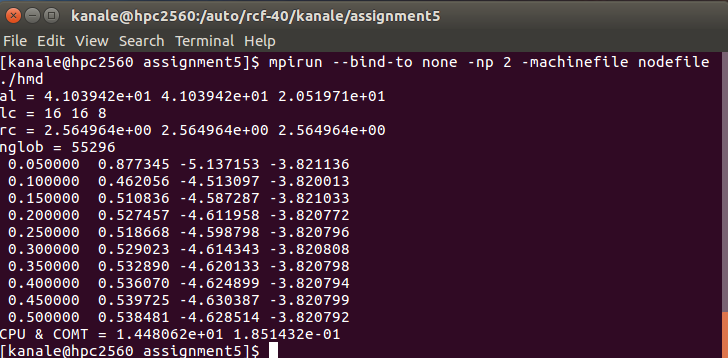
\includegraphics[scale=0.6]{output2.png}
 	\caption{Output for task 2-- Verification}
\end{figure}

\section{Task III-- Scalability}
In this task, the scalability of the program is tested w.r.t the number of threads. The plot is attached below.
\begin{figure}[!htbp]
	\centering
	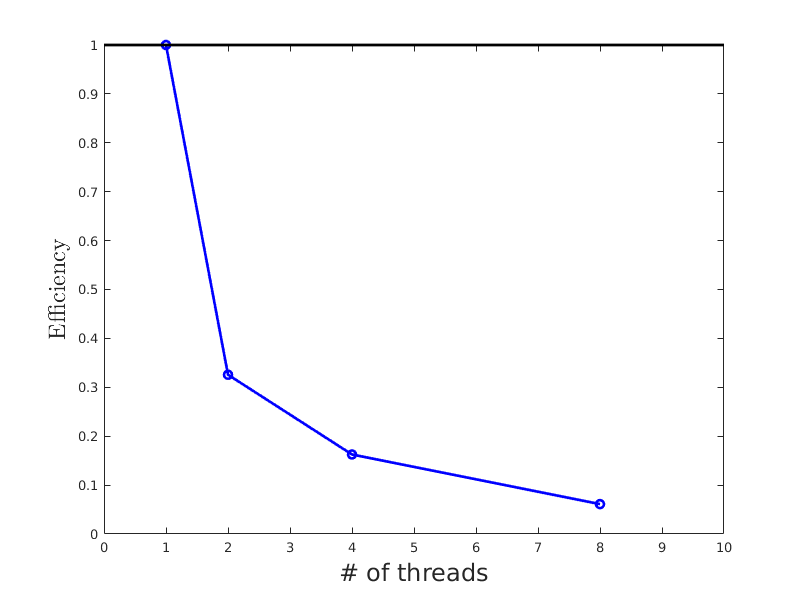
\includegraphics[scale=0.4]{scaling.png}
	\caption{Output for task 3-- Scaling}
\end{figure}


\appendix
\section{Appendix-- \texttt{hmd.c}}
\lstinputlisting{hmd.c}

\end{document}